\chapter{Perancangan}
\label{chap:perancangan}

Pada bab ini akan dijelaskan perancangan program yang dibuat pada penelitian ini. Perancangan terdiri dari masukan program, dan aktivitas sistem.

\section{Rancangan Antarmuka}
\label{sec:rancanganAntarmuka}

\subsection{Rancangan Antarmuka Formulir Data Baru Umat}
\label{sec:subRancanganAntarmuka}

\begin{figure}[H]
	\centering
	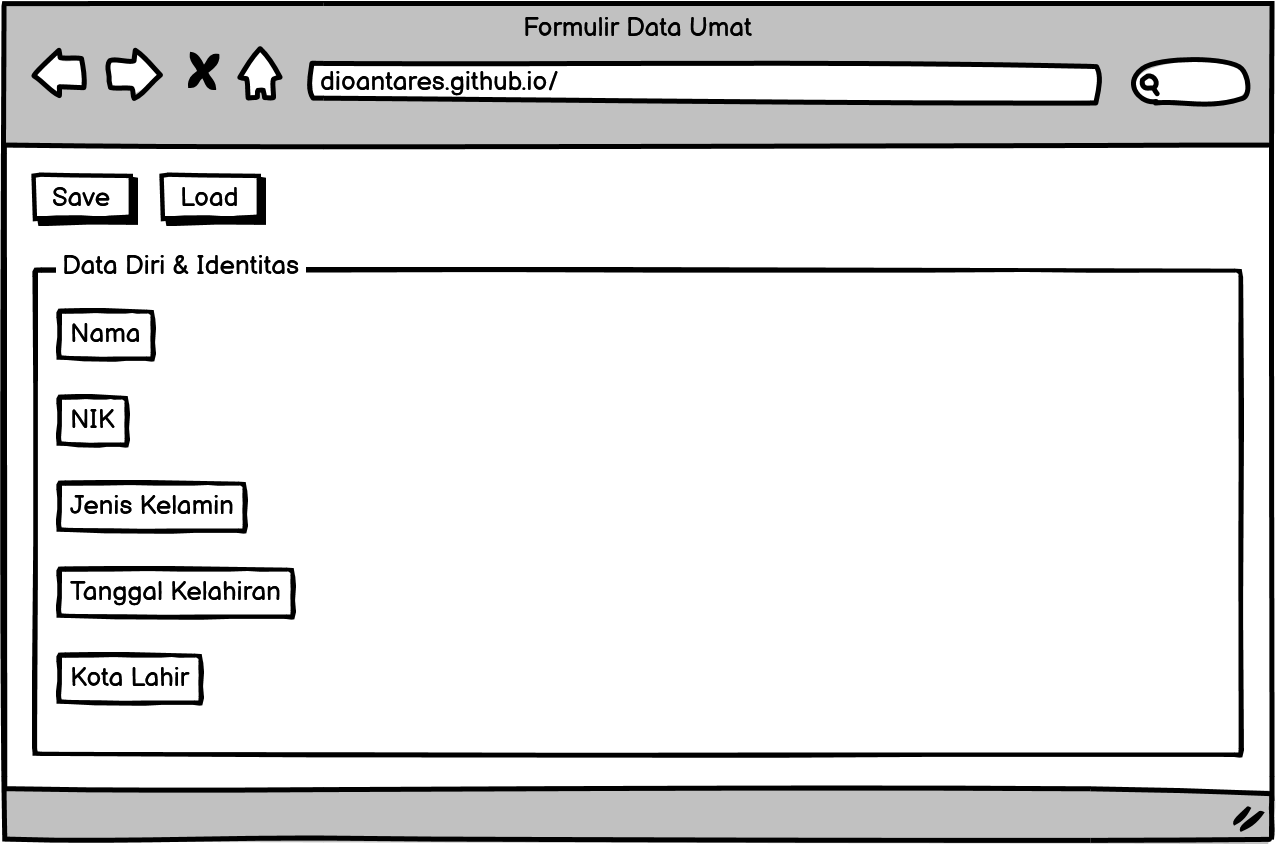
\includegraphics[scale=0.7]{Gambar/mockUpWebsite.png}
	\caption{Rancangan antarmuka halaman Formulir Data Umat} 
	\label{fig:formDataUmat}
\end{figure}

Seluruh fitur akan diimplementasikan pada halaman website yang berisikan formulir data umat. Gambar \ref{fig:formDataUmat} menunjukkan rancangan antarmuka halaman formulir data umat. Pada halaman formulir data umat sudah terdapat fitur save, load, submit, dan akan ada  beberapa perubahan pada rancangan baru formulir data baru umat, contoh perubahan tersebut adalah : 

\begin{enumerate}
	\item Halaman formulir dapat dibuka di mobile dengan baik \textit{(responsive design)}.
	\item Memunculkan keyboard yang tepat untuk input tertentu (contoh: nomor telepon menggunakan keypad)
	\item Menyimpan data secara otomatis di penyimpanan lokal, sehingga saat dibuka kembali, umat dapat melanjutkan pengisian. Fitur ini telah diimplementasikan pada tombol \textit{save} dan \textit{load}.
\end{enumerate}

\newpage

\subsection{Fitur Save}
\label{sec:save}

Fitur tombol \textit{Save} pada halaman ini berfungsi untuk menyimpan data yang telah diisi oleh umat. Formulir ini berisikan cukup banyak \textit{field} untuk diisi, sehingga apabila formulir ini tertutup atau umat akan melanjutkannya nanti, data akan tersimpan pada \textit{cookies}.

\subsection{Fitur Load}
\label{sec:load}

Fitur tombol \textit{Load} pada halaman ini berfungsi untuk mengisi data secara otomatis yang telah diisi oleh umat, fitur ini akan berjalan apabila sebelumnya umat sudah mengisi data lalu menggunakan fitur \textit{Save}. Tujuan utama dari fitur \textit{Load} ini adalah untuk mengambil data lalu mengisikannya secara otomatis pada field yang telah tersediah, sehingga apabila umat melanjutkan mengisi formulir, waktu yang diperlukan tidak perlu lama karena data akan diambil dari \textit{cookies}.

\subsection{Fitur Submit}
\label{sec:submit}

Fitur tombol \textit{Submit} pada halaman ini berfungsi untuk mengubah data yang telah terisi menjadi \textit{qr code}. Penggunaan fitur ini bertujuan agar \textit{qr code} dapat dipindai oleh admin dan dimasukan ke sistem SIMU.

\section{Rancangan Kode Halaman Website Formulir}
\label{sec:rancanganKodeFormulir}

Pada tahapan ini, penulis akan melakukan rancangan kode sistem, akan dibuat rancangan tampilan halaman sistem. Perancangan ini dibuat mengacu dari spesifikasi kebutuhan yang terselesaikan pada tahapan latar belakang masalah. Rancangan tersebut menghasilkan tata letak untuk fungsi-fungsi yang berhubungan dengan tampilan dari sistem pembelajaran HTML, CSS, dan Script. 

\subsection{Menampilkan Halaman Utama}
\label{sec:index}

Website Formulir Data Umat memiliki file berupa \textit{index.html}, fungsi dari \textit{index.html} merupakan file yang berfungsi sebagai halaman pertama yang dilihat pengunjung atau pengguna ketika mereka mengunjungi sebuah situs website, dan biasanya berisi informasi tentang situs website tersebut, termasuk tujuan, konten, dan navigasinya. 

File \textit{index.html} ditulis dalam HTML, yang merupakan bahasa markup standar yang digunakan untuk membuat halaman website. HTML adalah singkatan dari Hypertext Markup Language, dan memungkinkan pengembang membuat teks, gambar, tautan, dan elemen lain yang dapat ditampilkan di browser web. HyperText Markup Language (HTML) digunakan pada pengembangan web untuk mengorganisir dan memformat dokumen. \cite{indexcssScript}


\subsection{Desain Interface Halaman Utama}
\label{sec:style}

Dalam membuat desain untuk mengatur halaman website, makan file \textit{style.css} akan digunakan untuk mengatur sedemikian rupa halaman yang akan dibuat. Cascading Style Sheets (CSS) adalah standar teknologi pengembangan dalam pengaturan halaman web untuk menambahkan
style seperti font, warna, jarak dan lainnya ke dokumen website. Penggunaan file textit{style.css} akan menghasilkan tata letak untuk fungsi-fungsi yang berhubungan dengan tampilan dari sistem pembelajaran HTML serta CSS. \cite{indexcssScript}

\subsection{Menjalankan Script Halaman Utama}
\label{sec:script}

Penggunaan script dalam membangun sebuah website sangatlah penting, dalam penulisan kode <script>, tag tersebut digunakan untuk menulis script, atau lebih tepatnya adalah untuk menyisipkan script (seperti JavaScript) pada sisi client, penulisan kode script dapat dilakukan langsung di dalam element <script> , ataupun menggunakan sumber file eksternal dengan attribute src (soure). Pada website Formulir Data Umat digunakan \textit{library qrcodejs-master}, fungsinya untuk merubah text yang sudah diinput oleh umat menjadi sebuah bentuk qr code.




